% Created by tikzDevice version 0.11 on 2018-04-10 10:19:56
% !TEX encoding = UTF-8 Unicode
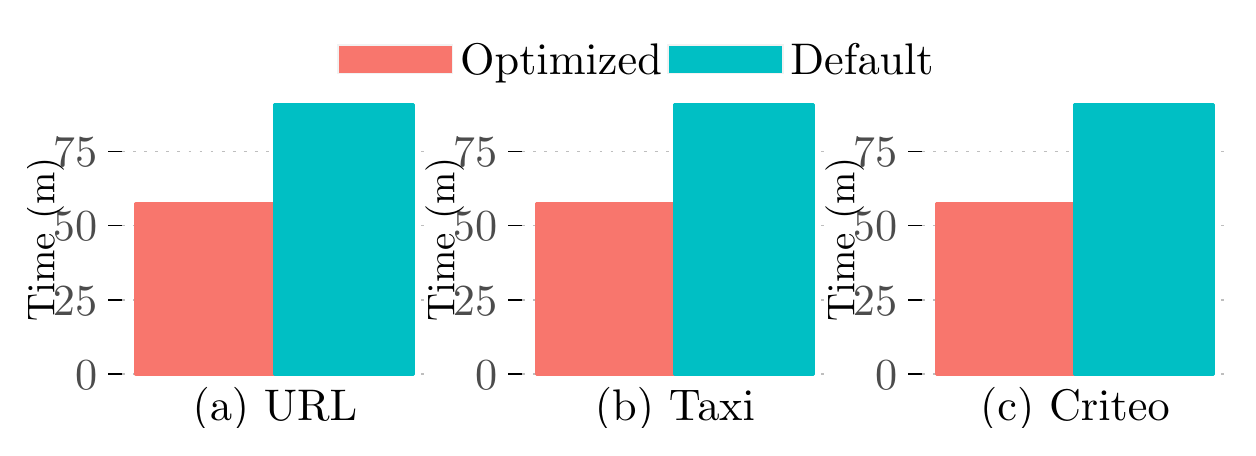
\begin{tikzpicture}[x=1pt,y=1pt]
\definecolor{fillColor}{RGB}{255,255,255}
\path[use as bounding box,fill=fillColor,fill opacity=0.00] (0,0) rectangle (433.62,144.54);
\begin{scope}
\path[clip] (  0.00,  0.00) rectangle (433.62,144.54);
\definecolor{fillColor}{RGB}{255,255,255}

\path[fill=fillColor] (101.43,121.66) rectangle (332.19,144.54);
\end{scope}
\begin{scope}
\path[clip] (  0.00,  0.00) rectangle (433.62,144.54);
\definecolor{drawColor}{RGB}{0,0,0}

\node[text=drawColor,anchor=base west,inner sep=0pt, outer sep=0pt, scale=  0.00] at (107.12,133.10) {Deployment};
\end{scope}
\begin{scope}
\path[clip] (  0.00,  0.00) rectangle (433.62,144.54);
\definecolor{drawColor}{RGB}{255,255,255}
\definecolor{fillColor}{gray}{0.95}

\path[draw=drawColor,line width= 0.6pt,line join=round,line cap=round,fill=fillColor] (111.46,127.35) rectangle (154.14,138.85);
\end{scope}
\begin{scope}
\path[clip] (  0.00,  0.00) rectangle (433.62,144.54);
\definecolor{drawColor}{RGB}{248,118,109}
\definecolor{fillColor}{RGB}{248,118,109}

\path[draw=drawColor,line width= 1.1pt,line cap=round,fill=fillColor] (112.88,128.78) rectangle (152.71,137.43);
\end{scope}
\begin{scope}
\path[clip] (  0.00,  0.00) rectangle (433.62,144.54);
\definecolor{drawColor}{RGB}{255,255,255}
\definecolor{fillColor}{gray}{0.95}

\path[draw=drawColor,line width= 0.6pt,line join=round,line cap=round,fill=fillColor] (230.77,127.35) rectangle (273.45,138.85);
\end{scope}
\begin{scope}
\path[clip] (  0.00,  0.00) rectangle (433.62,144.54);
\definecolor{drawColor}{RGB}{0,191,196}
\definecolor{fillColor}{RGB}{0,191,196}

\path[draw=drawColor,line width= 1.1pt,line cap=round,fill=fillColor] (232.19,128.78) rectangle (272.02,137.43);
\end{scope}
\begin{scope}
\path[clip] (  0.00,  0.00) rectangle (433.62,144.54);
\definecolor{drawColor}{RGB}{0,0,0}

\node[text=drawColor,anchor=base west,inner sep=0pt, outer sep=0pt, scale=  1.60] at (156.30,127.59) {Optimized};
\end{scope}
\begin{scope}
\path[clip] (  0.00,  0.00) rectangle (433.62,144.54);
\definecolor{drawColor}{RGB}{0,0,0}

\node[text=drawColor,anchor=base west,inner sep=0pt, outer sep=0pt, scale=  1.60] at (275.61,127.59) {Default};
\end{scope}
\begin{scope}
\path[clip] (  0.00,  0.00) rectangle (144.54,121.66);
\definecolor{drawColor}{RGB}{255,255,255}
\definecolor{fillColor}{RGB}{255,255,255}

\path[draw=drawColor,line width= 0.6pt,line join=round,line cap=round,fill=fillColor] (  0.00,  0.00) rectangle (144.54,121.66);
\end{scope}
\begin{scope}
\path[clip] ( 34.13, 14.51) rectangle (144.54,121.66);
\definecolor{fillColor}{RGB}{255,255,255}

\path[fill=fillColor] ( 34.13, 14.51) rectangle (144.54,121.66);
\definecolor{drawColor}{RGB}{255,255,255}

\path[draw=drawColor,line width= 0.3pt,line join=round] ( 34.13, 32.79) --
	(144.54, 32.79);

\path[draw=drawColor,line width= 0.3pt,line join=round] ( 34.13, 59.60) --
	(144.54, 59.60);

\path[draw=drawColor,line width= 0.3pt,line join=round] ( 34.13, 86.41) --
	(144.54, 86.41);

\path[draw=drawColor,line width= 0.3pt,line join=round] ( 34.13,113.22) --
	(144.54,113.22);
\definecolor{drawColor}{RGB}{190,190,190}

\path[draw=drawColor,line width= 0.6pt,dash pattern=on 1pt off 3pt ,line join=round] ( 34.13, 19.38) --
	(144.54, 19.38);

\path[draw=drawColor,line width= 0.6pt,dash pattern=on 1pt off 3pt ,line join=round] ( 34.13, 46.19) --
	(144.54, 46.19);

\path[draw=drawColor,line width= 0.6pt,dash pattern=on 1pt off 3pt ,line join=round] ( 34.13, 73.00) --
	(144.54, 73.00);

\path[draw=drawColor,line width= 0.6pt,dash pattern=on 1pt off 3pt ,line join=round] ( 34.13, 99.81) --
	(144.54, 99.81);
\definecolor{drawColor}{RGB}{255,255,255}

\path[draw=drawColor,line width= 0.6pt,line join=round] ( 64.24, 14.51) --
	( 64.24,121.66);

\path[draw=drawColor,line width= 0.6pt,line join=round] (114.43, 14.51) --
	(114.43,121.66);
\definecolor{drawColor}{RGB}{248,118,109}
\definecolor{fillColor}{RGB}{248,118,109}

\path[draw=drawColor,line width= 1.1pt,line join=round,fill=fillColor] ( 39.15, 19.38) rectangle ( 89.34, 80.88);
\definecolor{drawColor}{RGB}{0,191,196}
\definecolor{fillColor}{RGB}{0,191,196}

\path[draw=drawColor,line width= 1.1pt,line join=round,fill=fillColor] ( 89.34, 19.38) rectangle (139.52,116.79);
\end{scope}
\begin{scope}
\path[clip] (  0.00,  0.00) rectangle (433.62,144.54);
\definecolor{drawColor}{gray}{0.30}

\node[text=drawColor,anchor=base east,inner sep=0pt, outer sep=0pt, scale=  1.60] at ( 25.13, 13.87) {0};

\node[text=drawColor,anchor=base east,inner sep=0pt, outer sep=0pt, scale=  1.60] at ( 25.13, 40.68) {25};

\node[text=drawColor,anchor=base east,inner sep=0pt, outer sep=0pt, scale=  1.60] at ( 25.13, 67.49) {50};

\node[text=drawColor,anchor=base east,inner sep=0pt, outer sep=0pt, scale=  1.60] at ( 25.13, 94.30) {75};
\end{scope}
\begin{scope}
\path[clip] (  0.00,  0.00) rectangle (433.62,144.54);
\definecolor{drawColor}{RGB}{0,0,0}

\path[draw=drawColor,line width= 0.6pt,line join=round] ( 29.13, 19.38) --
	( 34.13, 19.38);

\path[draw=drawColor,line width= 0.6pt,line join=round] ( 29.13, 46.19) --
	( 34.13, 46.19);

\path[draw=drawColor,line width= 0.6pt,line join=round] ( 29.13, 73.00) --
	( 34.13, 73.00);

\path[draw=drawColor,line width= 0.6pt,line join=round] ( 29.13, 99.81) --
	( 34.13, 99.81);
\end{scope}
\begin{scope}
\path[clip] (  0.00,  0.00) rectangle (433.62,144.54);
\definecolor{drawColor}{RGB}{0,0,0}

\node[text=drawColor,anchor=base,inner sep=0pt, outer sep=0pt, scale=  1.60] at ( 89.34,  2.49) {(a) URL};
\end{scope}
\begin{scope}
\path[clip] (  0.00,  0.00) rectangle (433.62,144.54);
\definecolor{drawColor}{RGB}{0,0,0}

\node[text=drawColor,rotate= 90.00,anchor=base,inner sep=0pt, outer sep=0pt, scale=  1.40] at (  9.64, 68.09) {Time (m)};
\end{scope}
\begin{scope}
\path[clip] (144.54,  0.00) rectangle (289.08,121.66);
\definecolor{drawColor}{RGB}{255,255,255}
\definecolor{fillColor}{RGB}{255,255,255}

\path[draw=drawColor,line width= 0.6pt,line join=round,line cap=round,fill=fillColor] (144.54,  0.00) rectangle (289.08,121.66);
\end{scope}
\begin{scope}
\path[clip] (178.67, 14.51) rectangle (289.08,121.66);
\definecolor{fillColor}{RGB}{255,255,255}

\path[fill=fillColor] (178.67, 14.51) rectangle (289.08,121.66);
\definecolor{drawColor}{RGB}{255,255,255}

\path[draw=drawColor,line width= 0.3pt,line join=round] (178.67, 32.79) --
	(289.08, 32.79);

\path[draw=drawColor,line width= 0.3pt,line join=round] (178.67, 59.60) --
	(289.08, 59.60);

\path[draw=drawColor,line width= 0.3pt,line join=round] (178.67, 86.41) --
	(289.08, 86.41);

\path[draw=drawColor,line width= 0.3pt,line join=round] (178.67,113.22) --
	(289.08,113.22);
\definecolor{drawColor}{RGB}{190,190,190}

\path[draw=drawColor,line width= 0.6pt,dash pattern=on 1pt off 3pt ,line join=round] (178.67, 19.38) --
	(289.08, 19.38);

\path[draw=drawColor,line width= 0.6pt,dash pattern=on 1pt off 3pt ,line join=round] (178.67, 46.19) --
	(289.08, 46.19);

\path[draw=drawColor,line width= 0.6pt,dash pattern=on 1pt off 3pt ,line join=round] (178.67, 73.00) --
	(289.08, 73.00);

\path[draw=drawColor,line width= 0.6pt,dash pattern=on 1pt off 3pt ,line join=round] (178.67, 99.81) --
	(289.08, 99.81);
\definecolor{drawColor}{RGB}{255,255,255}

\path[draw=drawColor,line width= 0.6pt,line join=round] (208.78, 14.51) --
	(208.78,121.66);

\path[draw=drawColor,line width= 0.6pt,line join=round] (258.97, 14.51) --
	(258.97,121.66);
\definecolor{drawColor}{RGB}{248,118,109}
\definecolor{fillColor}{RGB}{248,118,109}

\path[draw=drawColor,line width= 1.1pt,line join=round,fill=fillColor] (183.69, 19.38) rectangle (233.88, 80.88);
\definecolor{drawColor}{RGB}{0,191,196}
\definecolor{fillColor}{RGB}{0,191,196}

\path[draw=drawColor,line width= 1.1pt,line join=round,fill=fillColor] (233.88, 19.38) rectangle (284.06,116.79);
\end{scope}
\begin{scope}
\path[clip] (  0.00,  0.00) rectangle (433.62,144.54);
\definecolor{drawColor}{gray}{0.30}

\node[text=drawColor,anchor=base east,inner sep=0pt, outer sep=0pt, scale=  1.60] at (169.67, 13.87) {0};

\node[text=drawColor,anchor=base east,inner sep=0pt, outer sep=0pt, scale=  1.60] at (169.67, 40.68) {25};

\node[text=drawColor,anchor=base east,inner sep=0pt, outer sep=0pt, scale=  1.60] at (169.67, 67.49) {50};

\node[text=drawColor,anchor=base east,inner sep=0pt, outer sep=0pt, scale=  1.60] at (169.67, 94.30) {75};
\end{scope}
\begin{scope}
\path[clip] (  0.00,  0.00) rectangle (433.62,144.54);
\definecolor{drawColor}{RGB}{0,0,0}

\path[draw=drawColor,line width= 0.6pt,line join=round] (173.67, 19.38) --
	(178.67, 19.38);

\path[draw=drawColor,line width= 0.6pt,line join=round] (173.67, 46.19) --
	(178.67, 46.19);

\path[draw=drawColor,line width= 0.6pt,line join=round] (173.67, 73.00) --
	(178.67, 73.00);

\path[draw=drawColor,line width= 0.6pt,line join=round] (173.67, 99.81) --
	(178.67, 99.81);
\end{scope}
\begin{scope}
\path[clip] (  0.00,  0.00) rectangle (433.62,144.54);
\definecolor{drawColor}{RGB}{0,0,0}

\node[text=drawColor,anchor=base,inner sep=0pt, outer sep=0pt, scale=  1.60] at (233.88,  2.49) {(b) Taxi};
\end{scope}
\begin{scope}
\path[clip] (  0.00,  0.00) rectangle (433.62,144.54);
\definecolor{drawColor}{RGB}{0,0,0}

\node[text=drawColor,rotate= 90.00,anchor=base,inner sep=0pt, outer sep=0pt, scale=  1.40] at (154.18, 68.09) {Time (m)};
\end{scope}
\begin{scope}
\path[clip] (289.08,  0.00) rectangle (433.62,121.66);
\definecolor{drawColor}{RGB}{255,255,255}
\definecolor{fillColor}{RGB}{255,255,255}

\path[draw=drawColor,line width= 0.6pt,line join=round,line cap=round,fill=fillColor] (289.08,  0.00) rectangle (433.62,121.66);
\end{scope}
\begin{scope}
\path[clip] (323.21, 14.51) rectangle (433.62,121.66);
\definecolor{fillColor}{RGB}{255,255,255}

\path[fill=fillColor] (323.21, 14.51) rectangle (433.62,121.66);
\definecolor{drawColor}{RGB}{255,255,255}

\path[draw=drawColor,line width= 0.3pt,line join=round] (323.21, 32.79) --
	(433.62, 32.79);

\path[draw=drawColor,line width= 0.3pt,line join=round] (323.21, 59.60) --
	(433.62, 59.60);

\path[draw=drawColor,line width= 0.3pt,line join=round] (323.21, 86.41) --
	(433.62, 86.41);

\path[draw=drawColor,line width= 0.3pt,line join=round] (323.21,113.22) --
	(433.62,113.22);
\definecolor{drawColor}{RGB}{190,190,190}

\path[draw=drawColor,line width= 0.6pt,dash pattern=on 1pt off 3pt ,line join=round] (323.21, 19.38) --
	(433.62, 19.38);

\path[draw=drawColor,line width= 0.6pt,dash pattern=on 1pt off 3pt ,line join=round] (323.21, 46.19) --
	(433.62, 46.19);

\path[draw=drawColor,line width= 0.6pt,dash pattern=on 1pt off 3pt ,line join=round] (323.21, 73.00) --
	(433.62, 73.00);

\path[draw=drawColor,line width= 0.6pt,dash pattern=on 1pt off 3pt ,line join=round] (323.21, 99.81) --
	(433.62, 99.81);
\definecolor{drawColor}{RGB}{255,255,255}

\path[draw=drawColor,line width= 0.6pt,line join=round] (353.32, 14.51) --
	(353.32,121.66);

\path[draw=drawColor,line width= 0.6pt,line join=round] (403.51, 14.51) --
	(403.51,121.66);
\definecolor{drawColor}{RGB}{248,118,109}
\definecolor{fillColor}{RGB}{248,118,109}

\path[draw=drawColor,line width= 1.1pt,line join=round,fill=fillColor] (328.23, 19.38) rectangle (378.42, 80.88);
\definecolor{drawColor}{RGB}{0,191,196}
\definecolor{fillColor}{RGB}{0,191,196}

\path[draw=drawColor,line width= 1.1pt,line join=round,fill=fillColor] (378.42, 19.38) rectangle (428.60,116.79);
\end{scope}
\begin{scope}
\path[clip] (  0.00,  0.00) rectangle (433.62,144.54);
\definecolor{drawColor}{gray}{0.30}

\node[text=drawColor,anchor=base east,inner sep=0pt, outer sep=0pt, scale=  1.60] at (314.21, 13.87) {0};

\node[text=drawColor,anchor=base east,inner sep=0pt, outer sep=0pt, scale=  1.60] at (314.21, 40.68) {25};

\node[text=drawColor,anchor=base east,inner sep=0pt, outer sep=0pt, scale=  1.60] at (314.21, 67.49) {50};

\node[text=drawColor,anchor=base east,inner sep=0pt, outer sep=0pt, scale=  1.60] at (314.21, 94.30) {75};
\end{scope}
\begin{scope}
\path[clip] (  0.00,  0.00) rectangle (433.62,144.54);
\definecolor{drawColor}{RGB}{0,0,0}

\path[draw=drawColor,line width= 0.6pt,line join=round] (318.21, 19.38) --
	(323.21, 19.38);

\path[draw=drawColor,line width= 0.6pt,line join=round] (318.21, 46.19) --
	(323.21, 46.19);

\path[draw=drawColor,line width= 0.6pt,line join=round] (318.21, 73.00) --
	(323.21, 73.00);

\path[draw=drawColor,line width= 0.6pt,line join=round] (318.21, 99.81) --
	(323.21, 99.81);
\end{scope}
\begin{scope}
\path[clip] (  0.00,  0.00) rectangle (433.62,144.54);
\definecolor{drawColor}{RGB}{0,0,0}

\node[text=drawColor,anchor=base,inner sep=0pt, outer sep=0pt, scale=  1.60] at (378.42,  2.49) {(c) Criteo};
\end{scope}
\begin{scope}
\path[clip] (  0.00,  0.00) rectangle (433.62,144.54);
\definecolor{drawColor}{RGB}{0,0,0}

\node[text=drawColor,rotate= 90.00,anchor=base,inner sep=0pt, outer sep=0pt, scale=  1.40] at (298.72, 68.09) {Time (m)};
\end{scope}
\end{tikzpicture}
